\section{Background Introduction}
        There are 6,000 to 7,000 languages being used all over the world currently, but around half of the world's population are using the most important 15 languages. With the development of globalization, the whole world has changed deeply. The impact of this trend does not only exist in economy and society, but also in language and culture. Nowadays, with the continuous improvement of transportation and communication, most people are able to speak the second language besides the mother language, and the second language plays an important role in traveling abroad and international trade.
    \begin{figure}[!htbp]                                           %ÌùÒ»ÕÅͼƬµÄ³ÌÐò
        \centering
        \includegraphics[width = .8\textwidth]{introduction.jpg}        %¸Ä£¬Í¼Æ¬ÎļþµÄÃû³Æ
        \caption{The Distribution of Various Language}                                  
        \label{introduction}                                           
    \end{figure}

    The current geographical distribution of different languages in the world is shown in the figure \ref{introduction}. When considering the total number of language speakers, native speakers, the second language speakers and even the third language speakers should be taken into consideration. The language distribution is complex and diverse, so the statistics on the total number of languages are a complicated job. At present, many experts and scholars have conducted research in this area to explore whether the trend of language distribution tends to be simplification.
\section{The Description of Problem}   
\subsection{Problem One: Online Dating Matches  }  
           
    For the increase of the total number of language speakers, we divided them into native speakers and second language speakers for model building. For the geographical distribution of language speakers, we should not only consider the population increase in each country after 5 years, but also the number of speakers who moving to other countries. Analyzing of the various factors of the problem, we consider the problem how to select the site of the International Office in each country as a risk-based site selection analysis:
This problem can be divided into four parts:
    \begin{itemize}         %ûÓкÚÌå×ÖµÄ
      \item Establish an increase model of the total number of language speakers changed with time to predict the change in the total number of language speakers in the next 50 years.
      \item Establish linguistic geography distribution model changed with time and predict the change of the geographical distribution of the language speakers in the next 50 years.
      \item According to the geographical distribution of language speakers, select the international offices to maximize the profits of the office.
      \item Consider changes in the global communication methods and determine whether the number of international offices can be reduced.
    \end{itemize}

\subsection{Problem Two:  More Suitable Estimate of An Ideally Sized Choice Set}                 
    In order to make the prediction more accurate, our work is divided into the following four aspects:
        \begin{figure}[!htbp]                                       
        \centering
        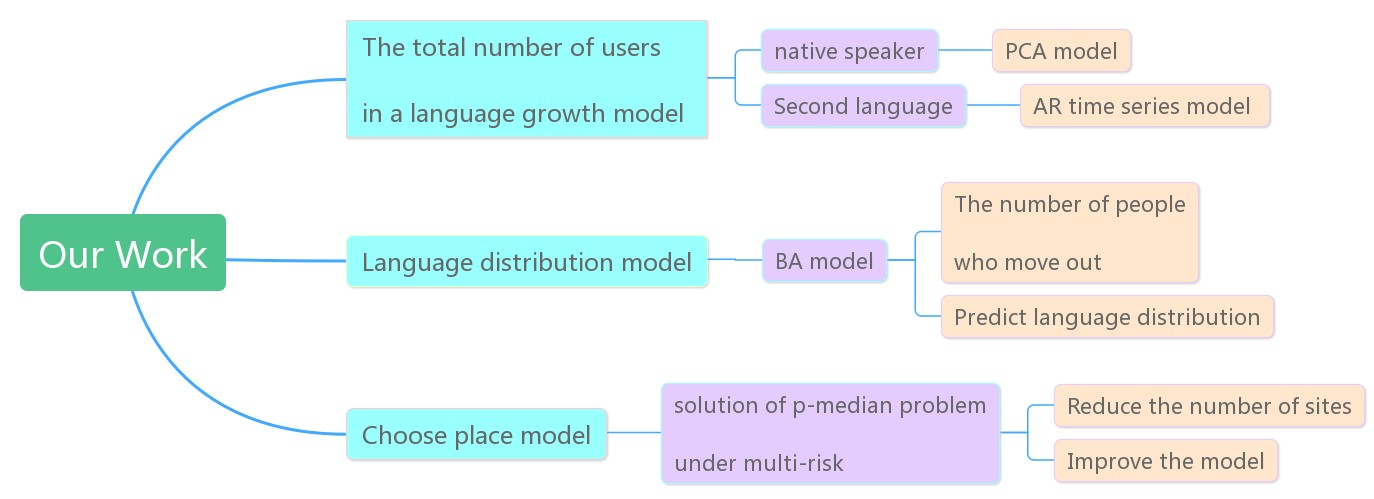
\includegraphics[width = .8\textwidth]{ourwork.jpg}      
        \caption{Flow Chart}                          
        \label{ourwork}                                      
    \end{figure}
\subsection{Problem Three: Information Forms Design and Effect Analysis Study}
1) To establish an increase model of the total number of language speakers, we should first obtain the number of native speakers in the future by predicting models of the population in different countries in the world. Secondly, we will determine the number of users who mainly use a certain language as a second language by determining the corresponding weights through principal component analysis .Finally, we will get the total of the two parts, and get the trend of the number of people who speak a certain language.\par 

2) Secondly, we use the scale-free network model to calculate the country's total value, according to the data function fitting. The FMR model is used to represent the point-to-point population mobility as the ratio of the nationals repulsive force to the attractive force of other countries .And we predict the migration pattern of the global population.\par 

3) Thirdly, we adopt the solution of p-median problem under multi-risk. We convert the multi-objective problem and the line-by-line weight problem into single-objective problem and then make fuzzy decision. Finally, we have found the location of six new international offices and give advises to clients.\par 

4) Finally, we submit a 2-page memo to summarize our findings and recommendations.\par 
\subsection{Problem Four:  Non-Technical News Release }

\section{Terminology Explained in Model}
    \begin{itemize}
      \item Nodes centrality degree: The number of edges connected to that node.
      \item L1 country: Countries referred to the country which has Russian as native language.
      \item L2 country: Countries referred to the country which has Russian as second language.
      \item L1 numbers: The numbers of native speakers of a certain language.
      \item L2 numbers: The numbers of second language speakers of a certain language.
    \end{itemize}


\section{Assumptions}
1. We assume that each country uses only the third and fourth languages with very few people, which has little effect on native speakers and second language speakers;

2. We do not consider small probability events in our model, assuming no random events such as world war and economic crisis.

3. Assuming that each country moves in and out of balance, that is, the total population does not change;

4. Assuming that the total number of immigrants to a country speaks the official language of the country and does not consider the issue of the offspring after the move;

5. Assume that all immigrants are legal immigrants;

6. Assuming that national policy does not change significantly over time;

7. Assumptions data are all true and reliable;

\section{Symbols and Definitions}
    \begin{table}[]
    \centering
    \caption{Symbols and Definitions}
    \begin{tabular}{llllll}
             \toprule
        \multicolumn{1}{c}{Symbols} & Meanings                                                                  \\
        \midrule
        ${Y_t}$                     & A country's L1 number                                                         \\
        $\Delta Y(t)$               & the number of population growth one year                                       \\
        $W(t)$                      & A country's L2 speakers                                                       \\
        $S(t)$                      & The population of the country                                                  \\
        ${O_i}$                     & The total degrees of country $i$                                               \\
        ${F_i}(t)$                  & \begin{tabular}[c]{@{}l@{}}The  thrust of\\   country $i$\end{tabular}       \\
        ${N_j}(t)$                  & The attractive force of country $i$                                            \\
        $N{`_i}(t)$                 & \begin{tabular}[c]{@{}l@{}}The tensile force\\   of country $i$\end{tabular}  \\
        ${Q_i}(t)$                  & The total number of people removed from country $i$                            \\
        $R$                         & The total expected value of a local profit                          \\
              \bottomrule
        \end{tabular}
    \end{table}

\section{Problem Solutions with Model Foundation}  
	\subsection{Solution for Problem One} 
	 \subsubsection{Justification of our approach}                              
For this question, the total population of a given language A is divided into two parts by us, which including those countries whose native language is A and those countries whose second(or 3rd,etc) language is A. Therefore, in order to find the accurate total numbers of speakers of language A, we should both find the two parts of the numbers of language A.

For the first part of the population, we investigate the population of a country where a language A is the mother tongue. However, not all people speak the native language. Therefore, we remove immigrants and people with a low level of literacy. As for population growth, we use the time series forecast model to make a prediction about the world's population.

For the second part of the population, we use PCA model to find the proportion of the numbers of speakers who have language A as a second language in a country(L2 country). According to the background of the title, we choose four factors to measure a country's level of learning a second language, which are cultural soft power, social pressure, immigration, the degree of opening up. Considering that if a government encourage people to learn second language, the trend of school learning is bound to upwards. So we regard the two factors language A promoted by the government and the language used in schools as one factor which is quantized by Primary Education Enrollment. We can use the per capital GDP as a measure of social pressure, because social pressure is inversely proportional to the level of consumption. The immigration is measured by net migration in a country. The degree of opening up is measured by the volume of export trade and the volume of import trade.

After confirming the factors, we use Principal Component Analysis(PCA) to analyze and get the corresponding weight of each factor, and find the relation between the final scores and the proportion of the numbers of speakers in L2 country. Finally, we sum up all the numbers of speakers in different country and compare the calculated data with the number of second-language speakers given in the question. Even though we did not count the third and fourth languages and ignored a few countries with small population, the results were slightly different but basically feasible.



            \begin{itemize}     %ÓкÚÌåС±êÌâµÄ
                \item \textbf{Why do we build the population growth model?}\\         %×¢Òâ¶ÎÄÚ»»ÐзûºÅ¼ÓÉÏÈ¥¹þ£¡
        If we want to model the distribution of language speakers in the future, building the population growth model is necessary because the numbers of different language speakers is changing over time. If we don`t consider this, we can not do the next step and the result must be unreliable.
                \item \textbf{Why do we divide each language into different country?}\\  % ×¢Òâ¶ÎÄÚ»»ÐзûºÅ¼ÓÉÏÈ¥¹þ£¡
        Because different country has different population growth rule and different L2 country has different proportion of L2 speaker. If we easily add up the native language and the second language and make a simple calculation of population growth model, the error of result is very big.
                \item \textbf{Why do we divide each language into two parts(L1 country, L2 country)?}\\
        It is obviously that L1 country and L2 country have different rule about calculating the proportion of the speakers of a particular language. So what we need do is to find the population of every country which speaks a particular language, and find the proportion of this language in these countries.
            \end{itemize}

    \subsubsection{Model 1: K-means}
    \subsubsection{Model 2: KNN}
    \subsubsection{Model 3: }
    1) AR Time Series Model

In order to get a model which have the ability to predict, we build an AR Time Series Model. Autoregressive model is:
\[\Delta {{\rm{Y}}_{\rm{t}}}{\rm{ = }}{\alpha _{\rm{0}}}{\rm{ + }}\sum\limits_{{\rm{i = 1}}}^n {{\alpha _i}\Delta {Y_{i - 1}} + {\mu _i}} \]


where ${{\alpha }_{0}}$. is constant, ${{\alpha }_{i}}$ is coefficient of the model, ${{\mu }_{i}}$ is White Noise Sequence.

As an analogy, the model of population growth is:

\begin{equation}\label{renkouzengzhang}
  {Y_t} = {Y_{t - 1}} + \Delta {Y_t}
\end{equation}
where ${{Y}_{t}}$ is the population this year, $\Delta {{Y}_{t-1}}$ is the number of population growth, $\left\{ \Delta {{Y}_{t}} \right\}$is first-order difference sequence of the population.

Based on this, the numbers of speakers of a particular language in L1 country are:
\[Y = (1 - \beta  - \lambda ){Y_t}\]
Where $\beta $ is the proportion of immigrant this year,$\lambda $ is the proportion of people with a low level of literacy. $n$is the number of L1 country.

2) PCA Model

    Second language, as a supporting language, can be obtained in different environments. Due to various influences such as immigration, national policies and cultural groups, people who speak a second language will change over time. Therefore, we selected four indicators of cultural soft strength, social pressure, immigration and the degree of opening up. The principal component analysis (PCA) model was used to derive the weight of each dependent variable and calculate the number of people using the second language in the country.

    \[\left\{ \begin{array}{l}
{F_1} = {a_{11}}{X_1} + {a_{12}}{X_2} + {a_{13}}{X_3} + {a_{14}}{X_4}\\
{F_2} = {a_{21}}{X_1} + {a_{22}}{X_2} + {a_{23}}{X_3} + {a_{24}}{X_4}\\
{F_3} = {a_{31}}{X_1} + {a_{32}}{X_2} + {a_{33}}{X_3} + {a_{34}}{X_4}\\
{F_4} = {a_{41}}{X_1} + {a_{42}}{X_2} + {a_{43}}{X_3} + {a_{44}}{X_4}\\
{F_5} = {a_{51}}{X_1} + {a_{52}}{X_2} + {a_{53}}{X_3} + {a_{54}}{X_4}
\end{array} \right.\]

Where  ${X_i}\left( {i = 1,2,3,4,5} \right)$ respectively represent the Secondary school enrolment rate, per capita GDP, net immigration, export trade and import trade.

Set ${{\widetilde{a}}_{ij}}$ as the value of index variable $j$ of model $i$.
\[{\widetilde a_{ij}} = \frac{{{a_{ij}} - {\mu _j}}}{{{s_j}}},(i = 1,...,5,j = 1,...,5)\]
\[{\widetilde x_j} = \frac{{{x_j} - {\mu _j}}}{{{s_j}}},(j = 1,...,5)\]

Where ${{\mu }_{j}}=\frac{1}{n}\sum\nolimits_{i=1}^{n}{{{a}_{i}}_{j}},{{S}_{j}}=\sqrt{\frac{1}{n-1}\sum\nolimits_{i=1}^{n}{{{({{a}_{i}}_{j}-{{\mu }_{i}})}^{2}}}}$
Then we calculate the correlation coefficient matrix $R={{({{r}_{ij}})}_{5*5}}$
\[{r_i}_j = \sum\nolimits_{k = 1}^n {\frac{{{{\widetilde a}_{ki}}*{{\widetilde a}_{kj}}}}{{n - 1}}} ,(i,j = 1,...,5)\]
Then, we calculate the eigenvalues ${{\lambda }_{j}}$ and the corresponding eigenvectors of $R$, to form the five new index variables. On the basis of the eigenvalues, we can get the contribution rate $b$ and the accumulative contributions rate $\alpha $of the parameters.
\[{b_j} = \frac{{{\lambda _j}}}{{\sum\nolimits_{k = 1}^m {{\lambda _k}} }},(j = 1,...,5)\]
\[{\alpha _p} = \frac{{\sum\nolimits_{k = 1}^p {{\lambda _k}} }}{{\sum\nolimits_{k = 5}^p {{\lambda _k}} }}\]

In descending order:$Z = {\alpha _1}{F_1} + {\alpha _2}{F_2} + ... + {\alpha _i}{F_i}$

We assume that there is a relation between the final scores and the proportion of the numbers of speakers in L2 country:
\[W(t) = \gamma Z(t)\]

Based on the available data, we find this weight and make a test which tell us it is feasible.

    3) Total Numbers of Speakers
    Total numbers of language speakers of a certain language is:
    \[S(t) = Y(t) + W(t)\]
\subsubsection{Solution and Result}
        In this problem we have to model the distribution of various language speakers over time. But due to the wide distribution of languages, we focus on the analysis of the four representative languages which are English, Russian, Chinese, Japanese. We use our model to predict their distribution ten years later.

For the growth of native languages speakers in these four languages, here is an example of analysis in Russian.

Figure.\ref{sub1} shows the autocorrelation and partial autocorrelation coefficients of Russia`s population growth function, and Figure.\ref{sub2} shows the population trend ten years after the prediction of Russia.

    \begin{figure}[!htbp]                                       % Ìù×óÓÒÁ½ÕÅͼƬµÄ³ÌÐò£¬ºÏÆðÀ´ÊÇÒ»ÕÅͼ£¬µ«ÊÇ£¨a£©£¨b£©·Ö¿ª
        \centering
        \subfloat[ACF and PACF]{                                %¸Ä£¬£¨a£©Í¼Æ¬ÔÚÎÄÕÂÖеıêÌâ
            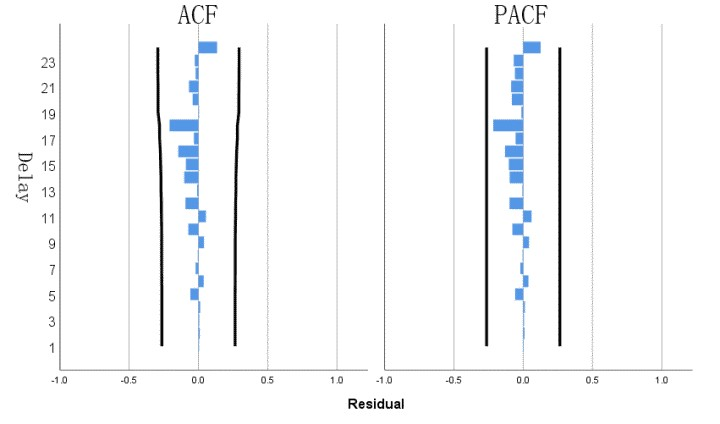
\includegraphics[width = .45\textwidth]{ACF.jpg}
            \label{sub1}                                           %¸Ä£¬£¨a£©Í¼Æ¬µÄ±êÇ©
        }
        \qquad
        \subfloat[Change in Russia`s Population]{                                %¸Ä£¬£¨b£©Í¼Æ¬µÄ±êÌâ
            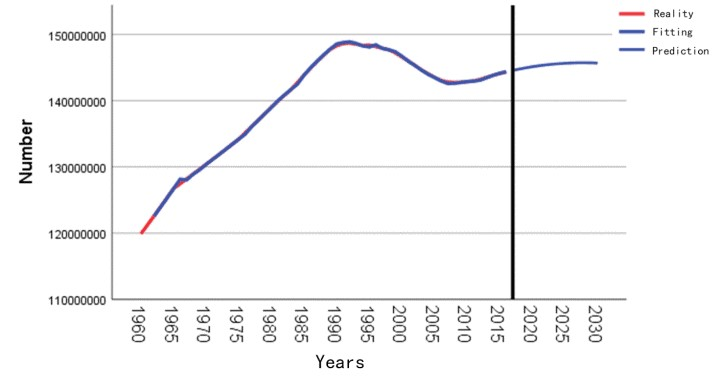
\includegraphics[width = .45\textwidth]{eluosi.jpg}
            \label{sub2}                                                %¸Ä£¬£¨b£©Í¼Æ¬µÄ±êÇ©
        }\\ %´Ë´¦ ¼Ó\\ºÍ»Ø³µ¿Õ³öÒ»ÐÐÊÇÒ»ÑùµÄЧ¹û¡£

        \caption{The Growth Model of Russia`s population}                                        %¸Ä£¬´óͼµÄ±êÌâ
        \label{eluosibijiaotu}                                           %¸Ä£¬´óͼµÄ±êÇ©
    \end{figure}

As can be seen from Figure.\ref{eluosibijiaotu}, Russia's total population is 145 million after 10 years. As for $\beta $, $\lambda $ parameter in Equation.\ref{renkouzengzhang}, we find the data from 1960 to 2016 in World bank.

We choose four languages and make a prediction about their L1 speakers number. Result is shown in Table.\ref{Atu}
\begin{table}[H]
\centering
\caption{The Change of L1 Speakers in Four Countries}
\label{Atu}
\begin{tabular}{llllll}
\cline{1-3}
\multicolumn{1}{c}{}        & \multicolumn{1}{c}{Now} & \multicolumn{1}{c}{In ten years} &  &  &  \\ \cline{1-3}
\multicolumn{1}{c}{Russian} & \multicolumn{1}{c}{153} & \multicolumn{1}{c}{162}             &  &  &  \\
\multicolumn{1}{c}{English} & \multicolumn{1}{c}{371} & \multicolumn{1}{c}{405}             &  &  &  \\
\multicolumn{1}{c}{Chinese} & \multicolumn{1}{c}{897} & \multicolumn{1}{c}{955}             &  &  &  \\
\multicolumn{1}{c}{Jpanese} & \multicolumn{1}{c}{128} & \multicolumn{1}{c}{124}             &  &  &  \\ \cline{1-3}

\end{tabular}
\end{table}

As for the number of L2 speakers, we almost find all the certain language`s L2 country and use our model to calculate the number of their L2 speakers in 2017, as is shown in Figure.\ref{AtuL2}. Comparing the result with the actual data in 2017, we find it that our model can basically figure out the number of L2 speakers.
    \begin{figure}[H]                                           %ÌùÒ»ÕÅͼƬµÄ³ÌÐò
        \centering
        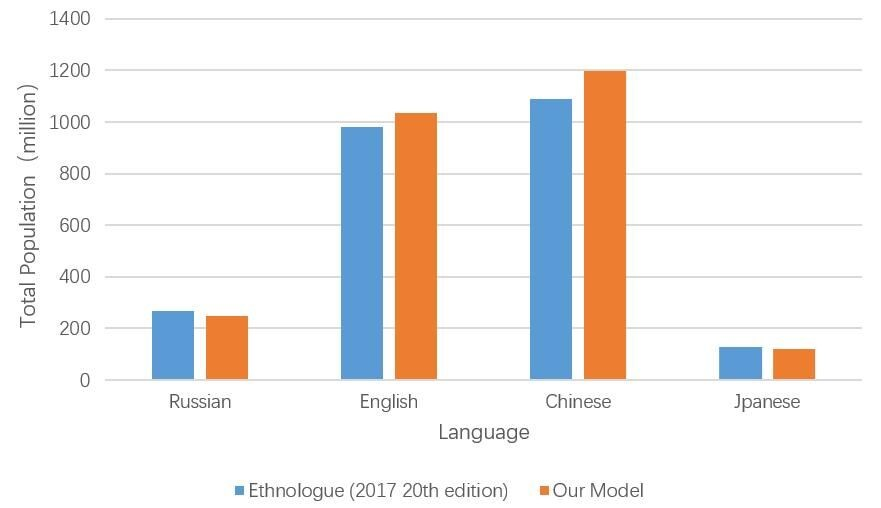
\includegraphics[width = .8\textwidth]{AtuL2.jpg}        %¸Ä£¬Í¼Æ¬ÎļþµÄÃû³Æ
        \caption{Model Test}                            %¸Ä£¬Í¼Æ¬ÔÚÎÄÕÂÖÐÏÔʾµÄÃû³Æ
        \label{AtuL2}                                           %¸Ä£¬Í¼Æ¬ÔÚ³ÌÐòÖеÄÃû³Æ£¬ÒýÓõÄʱºòÓÃ
    \end{figure}

Finally, we predict the total languages speakers of the four languages we choose.

\begin{table}[H]
\centering
\caption{The Total Numbers of Four Languages}
\label{Bjieguo}
\begin{tabular}{cccclcl}
            \toprule
                     & Native Language      &                      & \multicolumn{2}{c}{Second Language}                     & \multicolumn{2}{c}{Total}                               \\
                     \midrule
                     & Now                  & In Ten Years         & Now                  & \multicolumn{1}{c}{In Ten Years} & Now                  & \multicolumn{1}{c}{In Ten Years} \\
Russian              & 153                  & 162                  & 113                  & \multicolumn{1}{c}{119}          & 266                  & \multicolumn{1}{c}{281}          \\
English              & 371                  & 405                  & 611                  & \multicolumn{1}{c}{666}          & 982                  & \multicolumn{1}{c}{1071}         \\
Chinese              & 897                  & 955                  & 193                  & \multicolumn{1}{c}{205}          & 1090                 & \multicolumn{1}{c}{1160}         \\
Jpanese              & 128                  & 124                  & 1                    & \multicolumn{1}{c}{1.2}          & 129                  & \multicolumn{1}{c}{125.2} \\
\bottomrule
\end{tabular}
\end{table}

It can be seen from Table.\ref{Bjieguo} that the total languages speaker change a little after 10 years.

\subsubsection{Result and Analysis}
The data given by the title shows that at present, the top five languages in all languages are Chinese, English, Hindi, Spanish and Arabic. After consulting the literature, we consider these countries' current total population, level of economic development, degree of opening to the outside world and other factors. We think the rankings of the top five will not change and we finally decide to rank the 6th to the 16th Language the total number of languages 50 years after. According to the first question predictive model, the results obtained are in Table.\ref{Bdaan}.

\begin{table}[H]
\centering
\caption{The Predictions of 6th-16th Language`s Total Numbers of Speakers}
\label{Bdaan}
\begin{tabular}{ccccccc}
        \toprule
           & \multicolumn{2}{c}{L1} & \multicolumn{2}{c}{L2} & \multicolumn{2}{c}{Total} \\
           \midrule
           & Now    & In 50 Years   & Now    & In 50 Years   & Now     & In 50 Years     \\
Malay      & 77     & 107           & 204    & 271           & 281     & 378             \\
Bengali    & 242    & 340           & 19     & 22            & 261     & 362             \\
Russian    & 153    & 183           & 113    & 158           & 267     & 341             \\
Portuguese & 218    & 297           & 11     & 16            & 229     & 313             \\
French     & 76     & 101           & 153    & 203           & 229     & 304             \\
Hausa      & 85     & 132           & 65     & 93            & 150     & 225             \\
Punjabi    & 148    & 192           &        &               & 148     & 192             \\
German     & 76     & 106           & 52     & 69            & 129     & 175             \\
Persian    & 60     & 84            & 61     & 85            & 121     & 169             \\
Japanese   & 128    & 164           & 1      & 1.3           & 129     & 165.3           \\
Swahili    & 16     & 22            & 91     & 131           & 107     & 153\\
\bottomrule
\end{tabular}
\end{table}
\subsubsection{Strength and Weakness}
We can compare this result with the ranking of Ethnologue in the previous years, and find that the top ten rankings of the total number of languages in previous years are also basically stable, which shows that the ranking of the total number of language users has not changed. The condition is related to many factors.
\subsection{Solution for Problem Two}

  1. The country corresponding to the top-ten language can be divided into two parts. Some countries have a small population but have developed economically. Some countries have an underdeveloped  economy but have a lager population base.
      \begin{itemize}
        \item As for the first kind of countries like America, they have strong comprehensive national strength so their native language has become world official language, the other country should learn their language to carry out business and other activities.
        \item As for the second kind of countries like China, their people have superiority, so the number of native language is hard to be exceeded by other countries.
      \end{itemize}

  2. Since the countries ranked after the tenth in the rankings are not economy powerhouse and have not a large population base, growth in both native speakers and second language speakers is not high.

      3. We have ignored the small probability events, such as national split, war, invasion by other countries and other factors, so population model is the ideal model, so there will be such a result.


With a total population of 224 countries and regions in the world, some countries have a small population and a few other countries has very few immigrants, the impact on the first 26 languages is very small. Therefore, we only discuss forty countries with large populations and high immigration rates including China, India, the United States, Indonesia, Brazil, Pakistan, Nigeria, Bangladesh, Russia, Japan, Mexico, Ethiopia, the Philippines, Vietnam, Egypt, Germany, Iran, Turkey, the Democratic Republic of the Congo, Thailand, France, Great Britain, Italy, South Africa, Myanmar, Tanzania, South Korea, Columbus, Spain, Kenya, Argentina, Ukraine, Uganda, Sudan, Algeria, Poland, Canada, Iraq, Morocco, Afghanistan. These 40 countries account for 85\% of the world's total population, while the remaining 15\% are in more than 180 countries. Each country has a small population and a small impact on the entire population. Therefore, it is reasonable to do so.

For this question, we use the one-year world population migration data we found( cite), using a BA network model to calculate the total degree ${{O}_{i}}$ of 40 countries. Based on the rank of ${{O}_{i}}$, we stratify the 40 countries into four layers. We calculate the Data function parameter by using the data we have found in World Bank. Finally we get the four function of the total immigrant population of each country
 
    1) BA Model

   We select the top 10 countries in these 40 countries by the total degree. Then we use giving weights method to assign them 10 to 1, to indicate the score in this weighting network. The country with ordinate as the outflow of countries, the abscissa for the inflow country, enter the top 10 of the relationship data.

Nodes centrality degree is expressed as the number of edges connected to that node. In this paper, for a country which has indegree and outdegree, can be simplified as directed weighted network.

Definition ${{T}_{ij}}$ is the coefficient of the population that flows from country $i$ to country $j$, ${{T}_{ji}}$ indicates the opposite vector value.
\[{R_i} = \sum\limits_j {{T_{ji}}} \]
\[{C_i} = \sum\limits_j {{T_{ij}}} \],

 where ${{R}_{i}}$ indicate the indegree of country $i$ and ${{C}_{i}}$ indicate the outdegree of country $i$, There are directions in the network, and there will be no equal flow of population between countries, therefore ${{T}_{ij}}\ne {{T}_{ji}},{{R}_{i}}\ne {{C}_{i}}$.

In order to study the connection strength and flow strength of nodes in a network, we define ${{O}_{i}}={{R}_{i}}+{{C}_{i}}$ as the total degree of a node which is regarded as the degree of the node being in the center of the network.

    \begin{figure}[H]                                           %ÌùÒ»ÕÅͼƬµÄ³ÌÐò
        \centering
        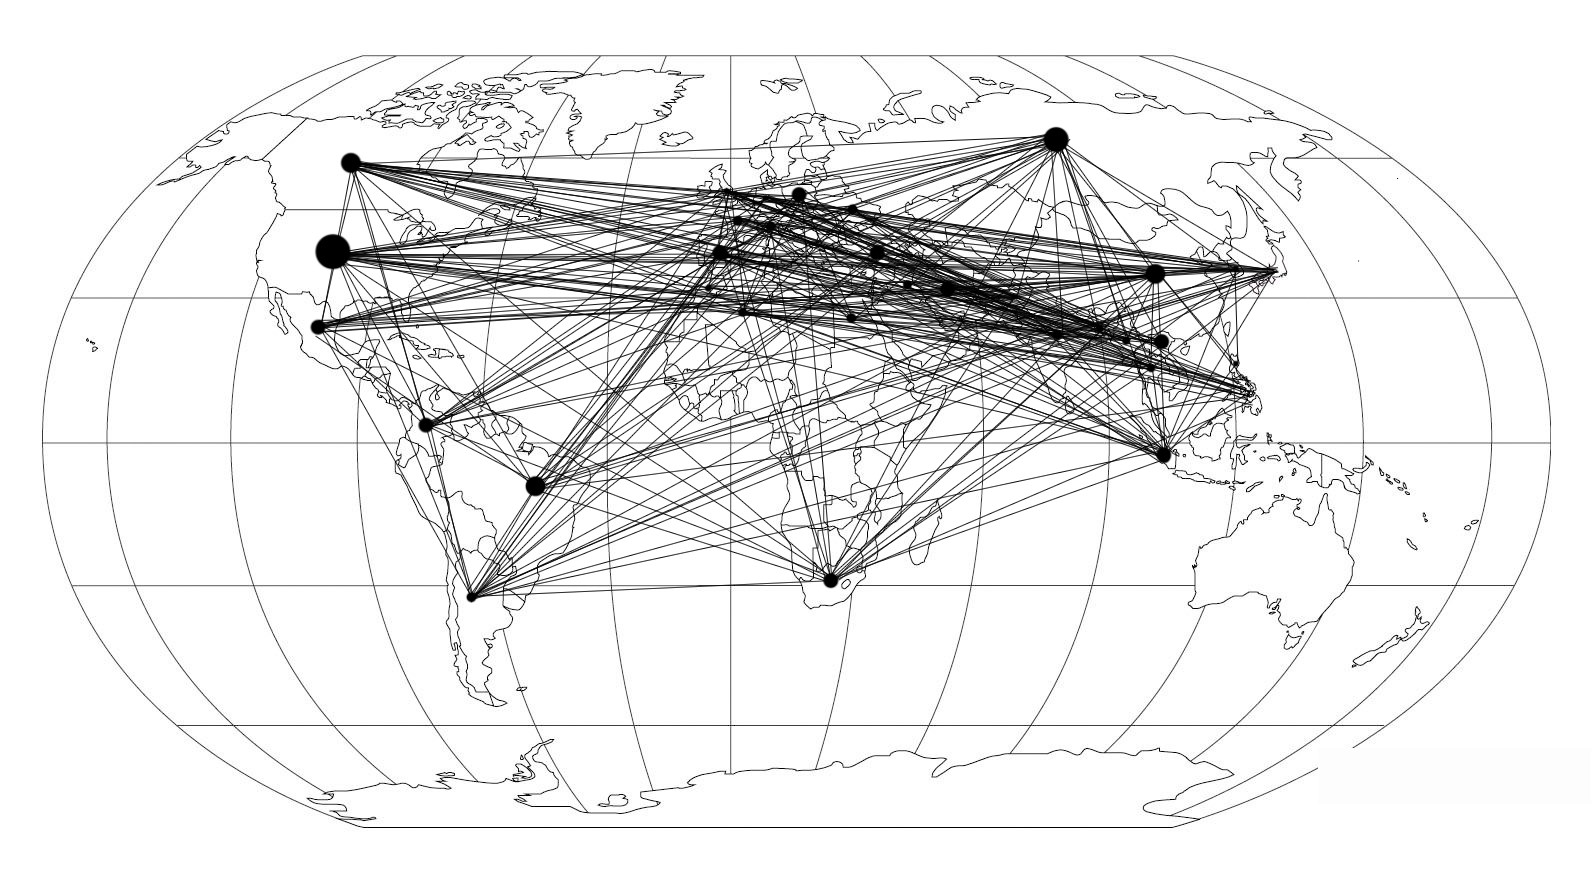
\includegraphics[width = .8\textwidth]{yiduixian.jpg}        %¸Ä£¬Í¼Æ¬ÎļþµÄÃû³Æ
        \caption{Global Population Mobility Network Space Pattern}                            %¸Ä£¬Í¼Æ¬ÔÚÎÄÕÂÖÐÏÔʾµÄÃû³Æ
        \label{yiduixian}                                           %¸Ä£¬Í¼Æ¬ÔÚ³ÌÐòÖеÄÃû³Æ£¬ÒýÓõÄʱºòÓÃ
    \end{figure}

According to the rankings of all national nodes ${O_i}$, it is found that the inter-country population mobility network shows a clear hierarchical level. In order to enhance the homogeneity of countries in the same level and the differences between different levels, we divided the 40 countries into four levels using the natural breakpoint classification method as is shown in Table.\ref{ceng}.
\begin{table}[H]
\centering
\caption{The Different Layer of The Forty Countries}
\label{ceng}
\begin{tabular}{ccccccclll}
                        \toprule
Hierarchy                & \multicolumn{5}{c}{Country}                                   \\
\midrule
The First Network Layer  & America      & Mexico      & Russian     & Ukraine  & India     \\
                         & Germany      & China       &             &          &          \\
                       \midrule
The Second Network Layer & Bangladesh   & Pakistan    & U.K         & France   & Canada    \\
                         & Italy        & Philippines & Iran        &          &           \\
                         \midrule
The Third Network Layer  & Turkey       & Spain       & Afghanistan & Algeria  & Poland   \\
                         & Morocco      & Japan       & Viet Nam    & Korea    &           \\
                         \midrule
The Forth Network Layer  & Brazil       & Colombia    & Argentina   & Iraq     & Congo   \\
                         & South Africa & Nigeria     & Thailand    & Tanzania & Myanmar   \\
                         & Indonesia    & Sudan       & Egypt       & Kenya    & Uganda   \\
                         & Ethiopia     &             &             &          &          \\
\bottomrule
\end{tabular}
\end{table}

\subsection{Solution for Problem Three}
We design a form to collect the necessary information. We use this information to build user profiles and base on this information to recommend dating partner to users.\par 
This information contains five parts:
\begin{itemize}
	\item User's photo: The user must show his face in the photo.
	\item Basic information of the user: For instance, user's name or nickname and so on. See appendix A for details.
	\item User social attribute information: For instance, user's family number and so on. See appendix A for details.
	\item Information about ideal dating partner: For instance, the gender of dating partner and so on. See appendix A for details. 
	\item Information about user character: We design a lot of multiple choice questions to test the user's personality. See appendix A for details.
\end{itemize}
\par 
In life, when someone ask our what date partner we want to date, we usually use a lot of words to describe the date partner's character. For married people, personality compatibility between husband and wife has a great influence on the quality of marriage\cite{1}.So, we set up a lot of questions to analyze the user's personality in detail.Some domestic research shows that the similarities and differences between couples' character have on significant effect on the quality of marriage. But dissatisfaction with the character of the spouse is an important reason for the decline in the quality of marriage and even thee breakdown of marriage\cite{2}.So, we set up a lot of topics to analyze user preferences. We also set up some questions to get user's basic information, but this information is not the point.\par 

The answers to all questions on the questionnaire can be represented by numbers. So, we can build a matrix to describe the user. The user matrix will be our model's input.



\subsection{Solution for Problem Four}


\section{Conclusions}
   
\section{Future Work}

\begin{thebibliography}{99}               
    \bibitem{1} CHENG Zao-Huo, TAN Lin-Xiang, ZHAO Yong, et al. Spouse's Personality and Marital Quality[J]. Chinese Mental Health Journal, 2006, 20 (4): 268-271
    \bibitem{2} Li Ling-Jiang, Yang De-Sen. A control study on the personality of 100 couples in divorce proceedings[J]. Chinese Mental Health Journal, 1993, 007 (2):70-72
    \bibitem{3}
    \bibitem{4}
\end{thebibliography}

\begin{appendices}
	
	\section{First appendix}
	\appendix
	\begin{itemize}
		\item User basic information:
		\begin{enumerate}
			\item name/nickname
			\item I am a man/woman.
			\item How many children do you have?
			\item When were you born?
			\item Where do you live?
			\item What is your nation?
			\begin{itemize}
				\item white
				\item Hispanic/Latino
				\item black/African descent
				\item Asian/pacific islander
				\item Indian
				\item Chinese			
				\item native American
				\item Arabic/middle eastern
				\item Korean
				\item Japanese
				\item other
			\end{itemize}
			\item What best describes your religious beliefs or spirituality?
			\begin{itemize}
				\item christian
				\item Jewish
				\item Muslim
				\item Hindu
				\item Buddhist
				\item Sikh
				\item Shinto
				\item other
				\item spiritual
				\item but not religious
				\item neither religious nor spiritual
				\item Baha'i
				\item cao dai
				\item Confucianism
				\item Jainism
				\item christian science
				\item Rastafarianism
				\item Taoism
				\item Tokyoite
				\item Unitarian-universalism
				\item Scientology
				\item metaphysical
				\item pagan
				\item Wiccan
				\item new age
				\item prefer not to specify 
			\end{itemize}  
			\item Which describes your highest level of education?
			\begin{itemize}
				\item doctorate
				\item masters
				\item bachelors
				\item associates
				\item some college
				\item high school
			\end{itemize} 
			\item What is you job?
			\item What's your personal income?(Your matches won't see this.)
			\item How often do you smoke?
			\begin{itemize}
				\item never
				\item socially
				\item once a week
				\item few times a week
				\item daily
			\end{itemize}
			\item How often do you drink?
				\begin{itemize}
				\item never
				\item on special occasions
				\item once a week
				\item few times a week
				\item daily
			\end{itemize}
			\item How tall are you?
			\item What are you passionate about?
			\item What two or three things do you enjoy doing with you leisure time?
		\end{enumerate}
		\item User social attribute information.(Optional)
		\begin{enumerate}
			\item Family members
			\item Graduated school
		\end{enumerate}
		\item Information about ideal dating partner.
		\begin{enumerate}
			\item I am seeking a man/woman.
			\item I am looking for someone between the ages of xx-xx.
			\item How far should we search for your matches?  x miles.
			\item How important is the distance of your match?
			\begin{itemize}
				\item not at all important
				\item somewhat important
				\item very important
			\end{itemize}
		\end{enumerate}
		\item Information about user character.
		\begin{enumerate}
			\item How well dose this generally describe you?(Not at all / somewhat / very well)
			\begin{itemize}
				\item warm
				\item clever
				\item dominant
				\item outgoing
				\item quarrelsome
				\item stable
				\item energetic
				\item predictable
				\item affectionate
				\item intelligent
				\item attractive
				\item compassionate
				\item loyal
				\item witty
				\item sensitive
				\item generous
				\item sensual
				\item stylish			
				\item athletic
				\item overweight
				\item plain
				\item healthy
				\item sexy
				\item content
				\item patient
				\item passionate
				\item caring
				\item genuine
				\item vivacious
				\item wise
				\item bossy
				\item leader
				\item irritable
				\item kind
				\item aggressive
				\item outspoken
				\item opinionated
				\item restless
				\item romantic
				\item selfish
				\item stubborn
				\item I do things according to a plan.
				\item I take time out for others.
				\item I feel unable to deal with things.
				\item I love to help others.
				\item I seek adventure.
				\item I desire sexual activity.
				\item I often leave a mess in my room.
				\item I often carry the conversation to a higher level.
				\item I get stressed out easily.
				\item I often make others feel good.
				\item I am good at analyzing problems.
				\item I usually stand up for myself.
				\item I am easily discouraged.
				\item I can handle a lot of information.
				\item I waste my time.
				\item I catch on quickly.
				\item I usually wait for others to lead the way.
				\item I love order and regularity.
				\item I often do nice things for people.
				\item I get angry easily.
				\item My personal religious beliefs are important.
				\item I ask questions in search of information.
				\item I think it is important to continually try to improve myself.
				\item I care about the physical shape I'm in.
				\item I feel better when I am around other people.
				\item I try to accommodate the other person's position.
				\item I try to understand the other person.
				\item I try to be respectful of all opinions different from my own.
				\item I try to resolve conflict well.
			\end{itemize}
			\item How strongly do you agree or disagree with...?(Absolutely disagree / Neither agree nor disagree / Absolutely agree)
			\begin{itemize}
				\item I am looking for a long-term relationship that will ultimately lead to marriage.
				\item When I get romantically involved, I tell my partner just about everything.
				\item It is difficult for me to let people get emotionally close to me.
				\item A "serious" relationship needs to be exclusive (i.e. monogamous).
				\item I know I can always count on the people who are closest to me.
				\item I don't need to have close relationships to be happy.
				\item Being monogamous helps build intimacy and trust in a romantic relationship.
				\item People often let you down if you depend on them.
				\item It's important for me to have close friends in my life.
				\item Being exclusive (i.e., monogamous) is one of benefits of being in a successful relationship.
				\item I sometimes find it difficult to trust people I get romantically involved with.
				\item I find it easy to get emotionally close to people.		
			\end{itemize}
			\item How important in a relationship is...(Not at all important / Somewhat important / Very important)
			\begin{itemize}
				\item My partner's dependability.
				\item My partner's sex appeal.
				\item My partner's physical appearance.
				\item Enjoying the way I feel around my partner.
				\item Our sexual compatibility.
				\item The friendship between me and my partner.
				\item Enjoying physical closeness with my partner.
				\item Being able to spend as much time as possible with my partner.
				\item Doing special things to let my partner know how important he/she is to me.
			\end{itemize}
			\item How happy are you with your physical appearance?
			\begin{itemize}
				\item Not at all
				\item Somewhat happy
				\item Very happy
			\end{itemize}
			\item How often in the past month have you felt...?(Really / Occasionally / Almost Always)
			\begin{itemize}
				\item Happy
				\item Sad
				\item Anxious
				\item Confident
				\item Hopeful
				\item Fearful about future
				\item Angry
				\item Calm
				\item Fortunate
				\item Out of control
				\item Fulfilled
				\item Depressed
				\item Unable to cope
				\item Satisfied
				\item Misunderstood
				\item Plotted against			
			\end{itemize}
			\item How skilled you are at the following things:(Not skilled / Somewhat Skilled / Very Skilled)
			\begin{itemize}
				\item Creating romance in a relationship
				\item Keeping physically fit
				\item Finding and taking on challenging activities
			\end{itemize}
			\item What's your interest in....?(None / Some Interest / Very Strong Interest)
			\begin{itemize}
				\item Watching movies
				\item Listening to music
				\item Watching TV
				\item Reading
				\item Parties
				\item Dining out
				\item Traveling
				\item Shopping
				\item Family
				\item Talking with friends
				\item Religious Community
				\item Religious Faith
				\item Conversation
				\item Hosting/Entertaining
				\item Church Involvement
			\end{itemize}
			\item If your best friends had to pick four words to describe you, which four from this list would they pick?
			\begin{itemize}
				\item good listener 
				\item modest
				\item respectful
				\item affectionate
				\item caring
				\item spontaneous
				\item physically
				\item fit
				\item warm
				\item outgoing
				\item optimistic
				\item dependable
				\item romantic
				\item creative
				\item loyal
				\item spiritual
				\item kind
				\item ambitious
				\item articulate
				\item rational
				\item easy-going
				\item generous
				\item happy
				\item quiet
				\item genuine
				\item intelligent
				\item sweet
				\item passionate
				\item energetic
				\item funny
				\item perceptive
			\end{itemize}
		\end{enumerate}
	\end{itemize}
	\begin{lstlisting}[language=python]


	
	\end{lstlisting}
\end{appendices}
